% id: 45-88
% book: 개념원리 공통수학2 · 04 직선의 방정식
% section: 연습문제 STEP 2
% figure: crop:fig-45-88.png
% answer: ⑤
% answer_source: 답지
% variant_level: 0 (원본 전사)
% 이 파일은 build.mjs 가 items.json 에서 만든다. 고칠 때는 items.json 을 고친다.
\smash{\raisebox{4.5mm}{\dmkichul{개념원리 공통수학2 45쪽 88번 · 교육청 기출}}}
\noindent\begin{minipage}[t]{0.58\linewidth}\vspace{0pt}\raggedright 그림과 같이 좌표평면에서 두 점~$\pt{A}(2{,}\mkern3mu\mathopen{}6)$, $\pt{B}(8{,}\mkern3mu\mathopen{}0)$에 대하여 일차함수 $y=\dfrac{1}{2}x+\dfrac{1}{2}$의 그래프가 $x$축과 만나는 점을 $\pt{C}$, 선분~$\pt{AB}$와 만나는 점을 $\pt{D}$라 할 때, 삼각형~$\pt{CBD}$의 넓이는?\end{minipage}\hfill\begin{minipage}[t]{0.4\linewidth}\vspace{0pt}\centering \setlength{\dmfigw}{94.0pt}\ifdim\dmfigw>\linewidth\setlength{\dmfigw}{\linewidth}\fi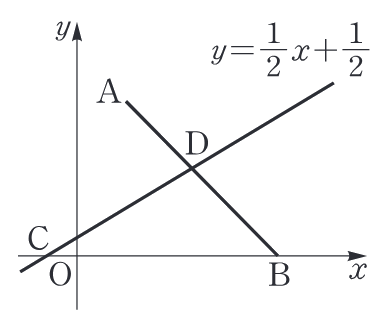
\includegraphics[width=\dmfigw]{figures/fig-45-88.png}\end{minipage}\par
\begin{choices32}{\rule[-3ex]{0pt}{8ex}$\dfrac{23}{2}$}{\rule[-3ex]{0pt}{8ex}$12$}{\rule[-3ex]{0pt}{8ex}$\dfrac{25}{2}$}{\rule[-3ex]{0pt}{8ex}$13$}{\rule[-3ex]{0pt}{8ex}$\dfrac{27}{2}$}\end{choices32}
